\documentclass[tikz,border=8pt]{standalone}
\usepackage{xcolor}
\usetikzlibrary{calc,arrows.meta,backgrounds}
\definecolor{bg}{HTML}{1B1F27}
\definecolor{fg}{HTML}{E6EDF3}
\definecolor{dim}{HTML}{9AA5B1}
\definecolor{c2}{HTML}{E5826F}
\definecolor{feat}{HTML}{F0C060}
\definecolor{cd}{HTML}{B39DDB}
\begin{document}
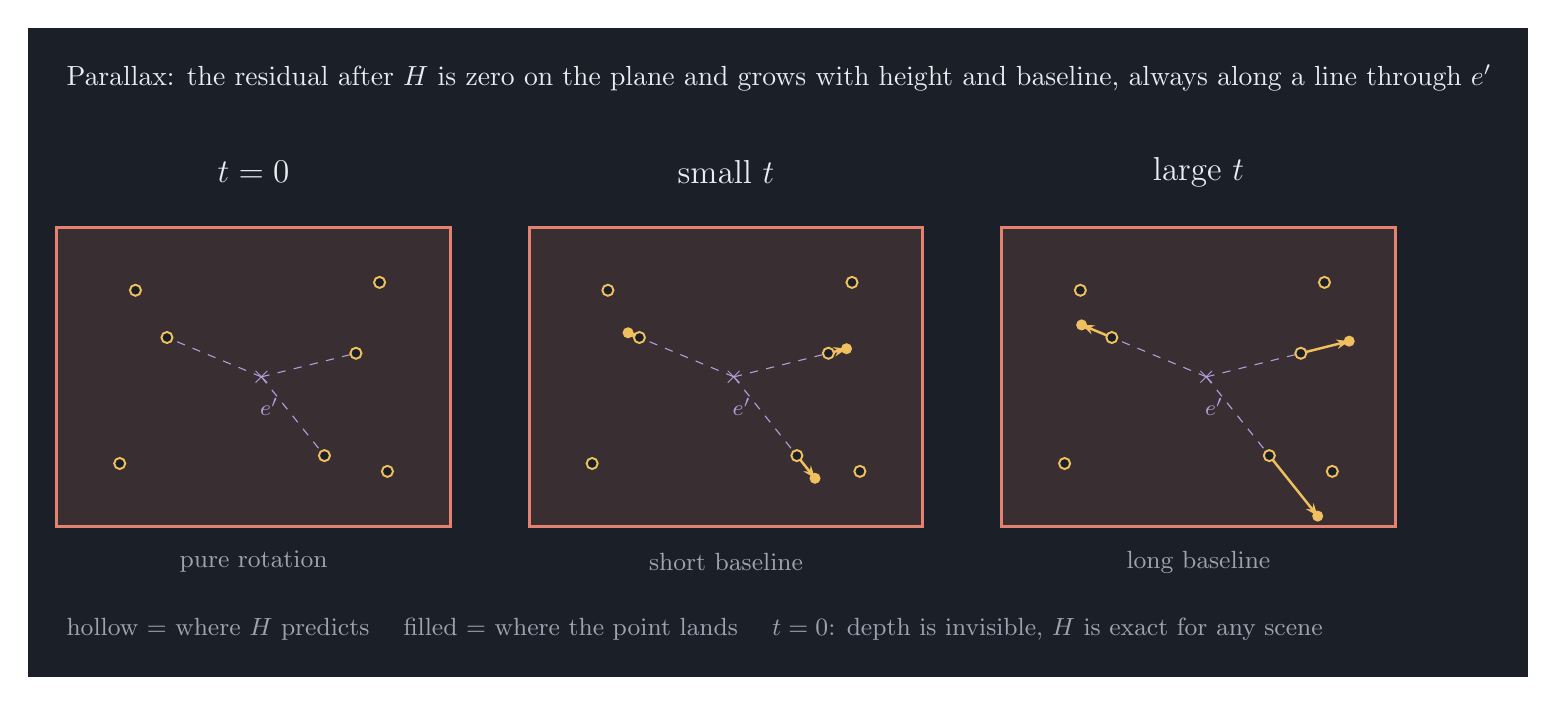
\begin{tikzpicture}[show background rectangle, background rectangle/.style={fill=bg}, inner frame sep=10pt, every node/.style={text=fg}]
\def\ex{2.6}\def\ey{1.9}
\foreach \ox/\s/\ttl/\sub in {0/0/{$t=0$}/{pure rotation},6/0.12/{small $t$}/{short baseline},12/0.32/{large $t$}/{long baseline}}{
  \draw[c2, line width=1pt, fill=c2!15!bg] (\ox,0) rectangle (\ox+5,3.8);
  \node[font=\large] at (\ox+2.5,4.5) {\ttl};
  \node[text=dim, font=\small] at (\ox+2.5,-0.45) {\sub};
  \node[text=cd, font=\small] at (\ox+\ex,\ey) {$\times$};
  \node[text=cd, font=\footnotesize] at (\ox+\ex+0.1,\ey-0.38) {$e'$};
  % px, py, height above the plane (0 = on the plane)
  \foreach \px/\py/\h in {0.8/0.8/0,1.0/3.0/0,4.1/3.1/0,4.2/0.7/0,1.4/2.4/1,3.8/2.2/1.6,3.4/0.9/2.4}{
    \pgfmathsetmacro{\ax}{\ox+\px}
    \pgfmathsetmacro{\bx}{\ox+\px+\s*\h*(\px-\ex)}
    \pgfmathsetmacro{\by}{\py+\s*\h*(\py-\ey)}
    \ifdim\h pt>0pt
      \draw[cd, dashed, line width=0.4pt] (\ox+\ex,\ey) -- (\ax,\py);
      \ifdim\s pt>0pt
        \draw[-{Stealth[length=1.6mm]}, feat, line width=0.9pt] (\ax,\py) -- (\bx,\by);
      \fi
    \fi
    \draw[feat, line width=0.7pt, fill=bg] (\ax,\py) circle (2pt);
    \ifdim\s pt>0pt
      \ifdim\h pt>0pt
        \fill[feat] (\bx,\by) circle (2pt);
      \fi
    \fi
  }
}
\node[anchor=west] at (0,5.7) {Parallax: the residual after $H$ is zero on the plane and grows with height and baseline, always along a line through $e'$};
\node[anchor=west, text=dim, font=\small] at (0,-1.3) {hollow = where $H$ predicts \quad filled = where the point lands \quad $t=0$: depth is invisible, $H$ is exact for any scene};
\end{tikzpicture}
\end{document}
